\documentclass{article}
\usepackage[utf8]{inputenc}
\usepackage{graphicx}
\usepackage{amsmath}

\title{CS 273: Machine Learning Final Project}
\author{Julius C Aguma (38208345), Matt Dees (30281707), James}
\date{December 2019}

\begin{document}

\maketitle

\section{Introduction}
\section{Dataset}
\section{Neural Network Models}

\par To analyse the capacity of neural network models on the fashion-mnist data, we chose to use a feedforward and convolutional neural network. While holding all other parameters constant, the number of hidden layers, $k$ was varied for values ${1,2,4,8}$. Results of this analysis are presented below with a summary of the architectures of both models.

\subsection{FeedForward model}
\subsubsection{Architecture}
\par Using tensorflow with keras, we built a feedforward network that takes fashion mnist data as input read through the mnist-reader.py script. The network has $k$ hidden layers where $k$ is varied for an analysis of capacity, that is a comparison of deep vs shallow networks on the fashion-mnist dataset. The data is split into training and validation data as shown in the model parameters below and the model is trained for 50 epochs where each epoch has 40000 iterations. In addition we use dropout factors less than 1 for regularization and cross entropy as loss function with the adadelta optimizer as a learning rate method for our gradient descent. The hidden layers use relu for an activation function while the output layer uses softmax. All inputs are normalized. Below are parameters and results for each $k$ in the set ${1,2,4,8}$
\clearpage
\begin{enumerate}
    \item  K = 1
        \begin{figure}[!ht]
            \begin{center}
                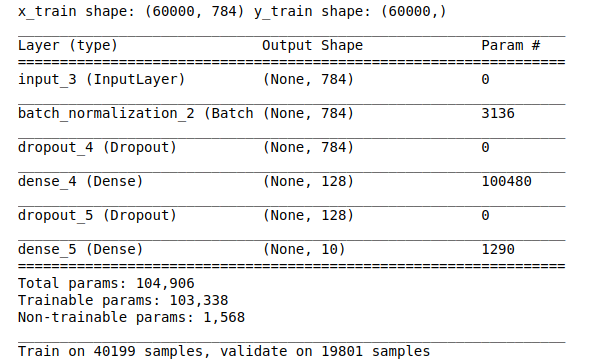
\includegraphics[width=1.0\textwidth]{1a.png}
            \end{center}
        \end{figure}
        \begin{figure}[!ht]
            \begin{center}
                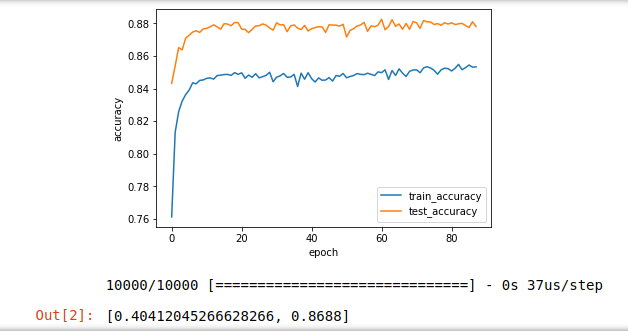
\includegraphics[width=1.0\textwidth]{1b.png}
            \end{center}
        \end{figure}
        \clearpage
    \item  K = 2
        \begin{figure}[!ht]
            \begin{center}
                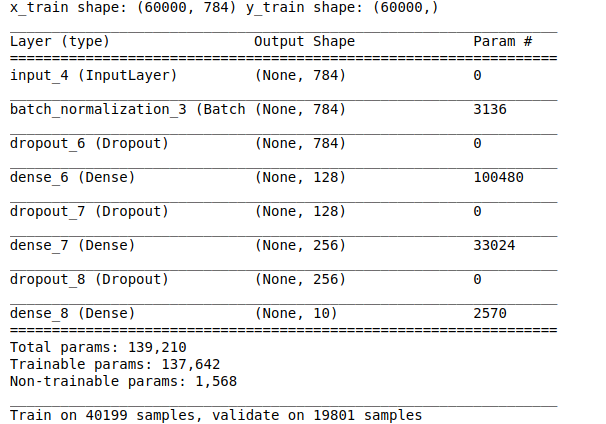
\includegraphics[width=1.0\textwidth]{2a.png}
            \end{center}
        \end{figure}
        \begin{figure}[!ht]
            \begin{center}
                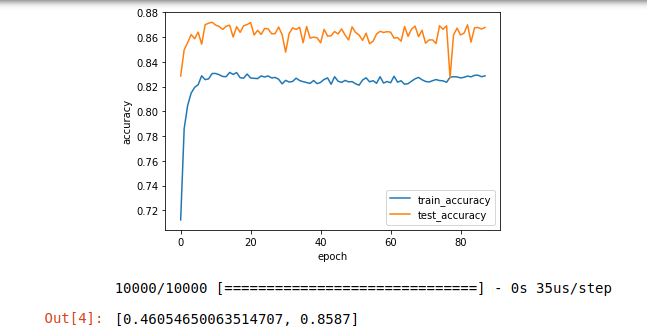
\includegraphics[width=1.0\textwidth]{2b.png}
            \end{center}
        \end{figure}
        \clearpage
    \item  K = 4
        \begin{figure}[!ht]
            \begin{center}
                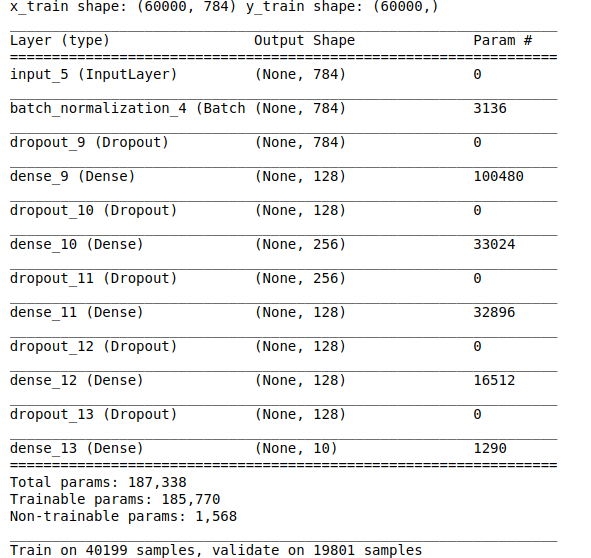
\includegraphics[width=1.0\textwidth]{4a.png}
            \end{center}
        \end{figure}
        \begin{figure}[!ht]
            \begin{center}
                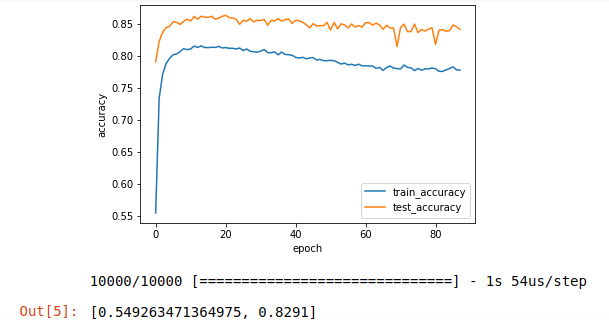
\includegraphics[width=1.0\textwidth]{4b.png}
            \end{center}
        \end{figure}
        \clearpage
    \item  K = 8
        \begin{figure}[!ht]
            \begin{center}
                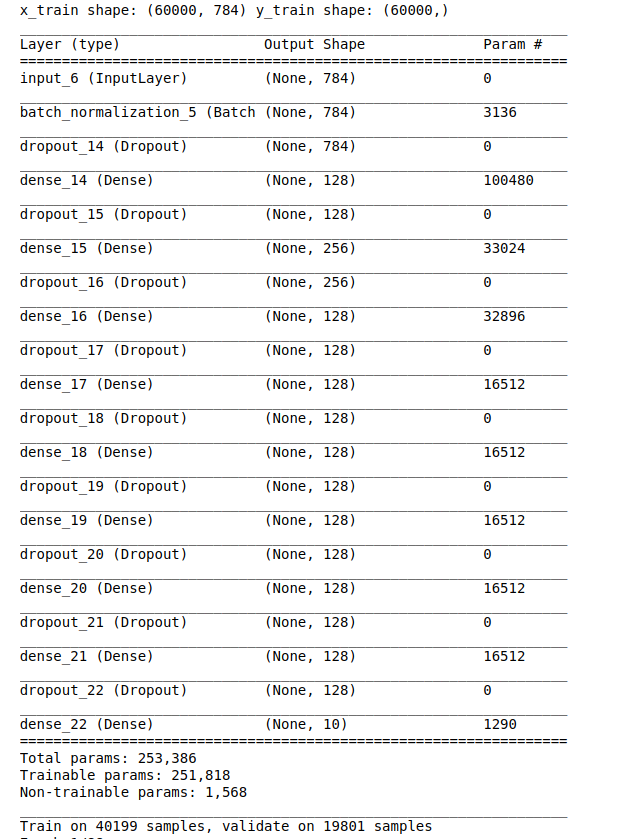
\includegraphics[width=1.0\textwidth]{8a.png}
            \end{center}
        \end{figure}
        \begin{figure}[!ht]
            \begin{center}
                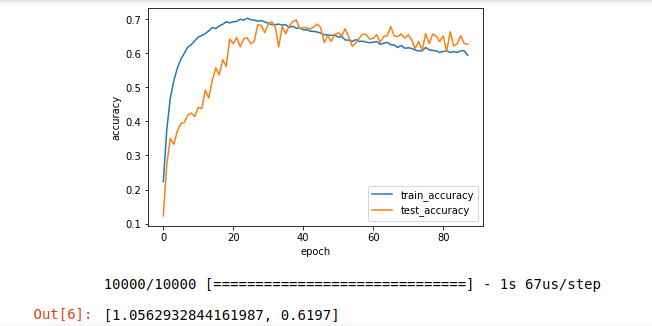
\includegraphics[width=1.0\textwidth]{8b.png}
            \end{center}
        \end{figure}
        \clearpage
\end{enumerate}

\subsection{Convolutional model}
\subsubsection{Architecture}
\par The convolutional model(cnn) is similar to the feedforward model in number of hidden layers, optimizer, regularization, activation functions, and validation. However, the  cnn also has 2 3x3 convolutional  filters and a 2x2 max pooling layer for downsampling the convolution layers. Results follow below.

\begin{enumerate}
    \item  K = 1
        \begin{figure}[!ht]
            \begin{center}
                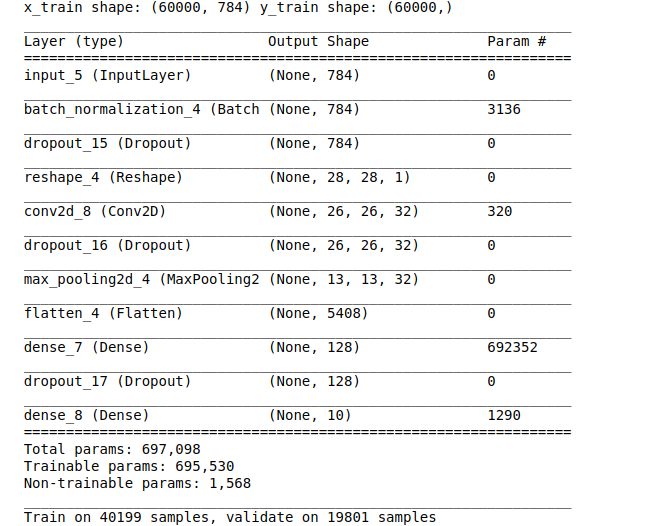
\includegraphics[width=1.0\textwidth]{ca.png}
            \end{center}
        \end{figure}
        \begin{figure}[!ht]
            \begin{center}
                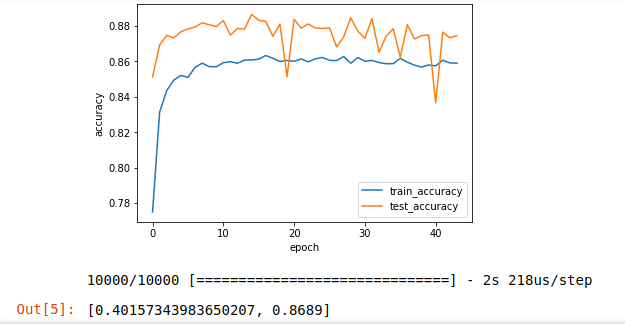
\includegraphics[width=1.0\textwidth]{cb.png}
            \end{center}
        \end{figure}
        \clearpage
    \item  K = 2
        \begin{figure}[!ht]
            \begin{center}
                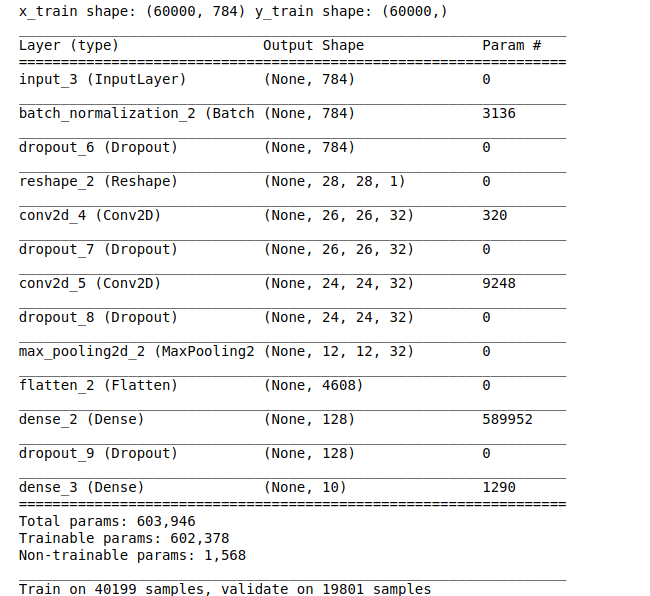
\includegraphics[width=1.0\textwidth]{c1a.png}
            \end{center}
        \end{figure}
        \begin{figure}[!ht]
            \begin{center}
                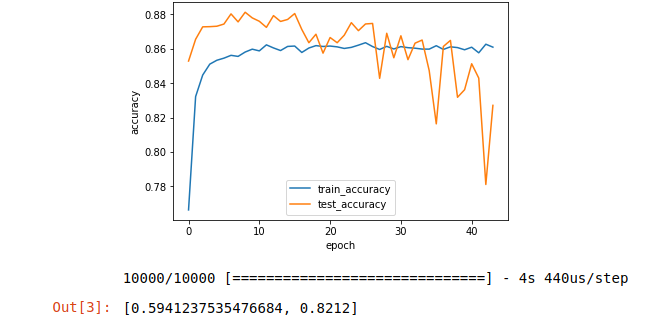
\includegraphics[width=1.0\textwidth]{c1b.png}
            \end{center}
        \end{figure}
        \clearpage
    \item  K = 4
        \begin{figure}[!ht]
            \begin{center}
                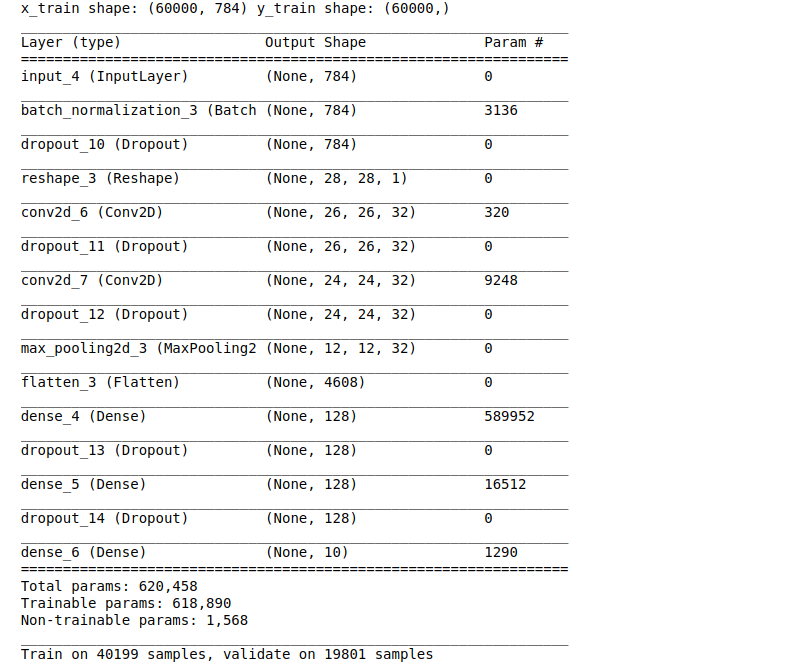
\includegraphics[width=1.0\textwidth]{c2a.png}
            \end{center}
        \end{figure}
        \begin{figure}[!ht]
            \begin{center}
                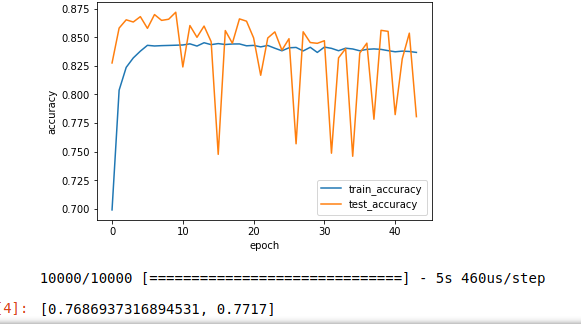
\includegraphics[width=1.0\textwidth]{c4b.png}
            \end{center}
        \end{figure}
        \clearpage
\end{enumerate}

\subsection{Discussion of results}
\par The feedforward model gave more consistent predictions with a smoother curve while the cnn gave us higher accuracy with a peak of about 90\%. For both architectures, the rate of overfitting increased with increase in the number of hidden layers. More so for the cnn where by k = 4 we see an overwhelming amount of overfitting. We also see that the peak accuracy never increased with increase in number of hidden layers. Further proving the known fact that capacity of a neural network doesnot increase with deeper networks but only the type of functions that can be estimated improves. A good next step in the capacity study would be to look at how the network performance changes with wider hidden layer, that is hidden layers with more neurons.
\end{document}

